%!TeX root=../tese.tex
%("dica" para o editor de texto: este arquivo é parte de um documento maior)
% para saber mais: https://tex.stackexchange.com/q/78101


% One of our working hypothesis is that a refactoring commit is only a refactoring commit, that is no new features have been added nor there are other code alterations in this single commit. Even if a refactoring commit has other alterations to the code base, those alterations may not be in the same file of the refactoring or even in the same function so with some processing we should be able to obtain ``pure'' refactoring commits for a reasonable portion of our dataset.


\chapter{(Re)Building a Dataset}
 Originally, this project was conceived as a partnership with the TUDelft where we would build upon their previous work by training our models on the dataset they build in \citet{mauricio_paper} and that we previously presented in Section~\ref{sec:mauricio_dataset}. However once we received the full dataset %, after months of wait,  
  we realized that it was not suitable for our needs. Since they did not capture any information regarding which lines were extracted in the function extractions nor any other more minute details about where and how  exactly the refactorings occurred, there was no way to train a supervised machine learning model. The dataset could still be used for unsupervised approaches and other less granular tasks, however we decided to collect our own dataset to be able to accomplish our original objectives. We briefly explored the possibility of leveraging the existing dataset to obtain the extracted lines but we reached the conclusion that scrapping them from scratch would be simpler and faster.
This heavily impacted our proposed timeline since there was a need to create an usable dataset from scratch. Utilizing a list of over 40.000 Java repositories %from\citet{lista_repos} 
provided by SERG - TUDelft, and made available at \citet{lista_repos},
we created a data pipeline with a tool called RefactoringMiner \citep{refactoringminer_2.0} at its core. 
In this chapter we will detail how we constructed this dataset and the reasoning behind some of our decisions, this new objective of creating a dataset instead of using a pre-built one led us to a series of new decisions. The first of them being our decision to maintain our objective of working with function extractions. 
If we reference Table~\ref{table:mau_refacs} one might notice that the most common refactoring was of the \textit{Rename Method} type. Although they were not originally published with this sole task or problem formulation in mind, code2vec, code2seq and code transformer achieve an impressive performance in this task \citep{code2vec, code2seq, code_transformer}.  In contrast, the second most common refactoring was of the type \textit{Extract Method} and to the best of our knowledge there is no model for automating this refactoring. Tackling this new and interesting task was the biggest motivator behind our choice of working with function extractions instead of other less common refactorings.

% \footnote{If the cohorts analyzed by \citet{mauricio_paper} are a big and general enough segment of Java projects to be considered representative of Java projects and/or Java programmers at large could be cause for debate, however investigating this would be out of the scope for this project.}

 This leads us to the next decision in our data building task, what tool should we use to obtain function extractions?


 \section{RefactoringMiner}


To create a model for automatic function extraction our dataset needs to have examples of function extractions with the lines extracted being appropriately tagged. Doing so by hand would be error prone and time consuming, so tools crafted to ``mine'' git repositories for such refactorings are commonly used.

One of such tools is RefactoringMiner 2.0. It can detect 40 different refactoring types through rules based on statement mapping information and AST node replacements. In its 1.0 version \citep{refactoring_miner1} it attained a state of the art performance and, maybe more importantly, introduced a refactoring oracle of validated refactoring instances, providing a new rigorous benchmark for the field. RefactoringMiner 2.0 expanded this oracle into 7,226 true positives in total, for 40 different refactoring types detected
by one (minimum) up to six (maximum) different tools. These refactorings were mined from 536 commits from 185 open-source Java projects hosted on GitHub.
Another important feature present in RefactoringMiner 2.0 is the ability to detect nested refactorings:

\begin{myquote}
\textit{A refactoring operation that takes place in code resulting from the application of another refactoring operation is a nested refactoring. For example, the renaming or extraction of local variables inside the body of an extracted method are nested refactoring operations[...].}
\\\citet{refactoringminer_2.0}
\end{myquote}

Fig.~\ref{img:nested_refac} shows a real case of nested extract method refactorings. 

\begin{figure}[!ht]
\centerline{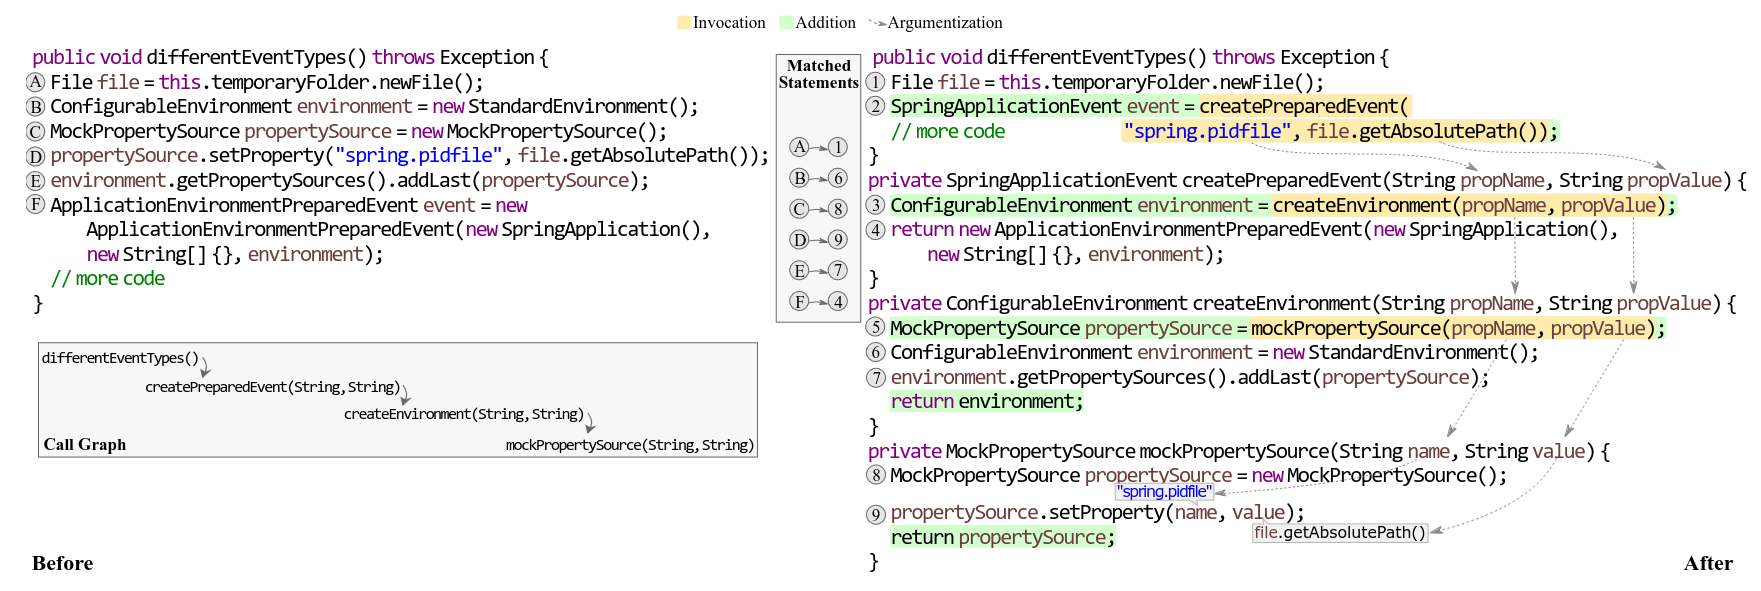
\includegraphics[width=1.2\textwidth]{figuras/nested_refacs.png}   }
\caption{Nested extract method refactorings mined from \url{github.com/spring-projects/spring-boot/commit/becce}. There
are 3 levels of nested extracted methods with each extracted
method calling the subsequent one. Image from \citet{refactoringminer_2.0}.}
\label{img:nested_refac}
\end{figure}

This tool is the same one utilized to create the dataset described in Section~\ref{sec:mauricio_dataset}, so when we were choosing a refactoring detection tool it was naturally considered. But with the release of new tools and versions we were interested if RefactoringMiner could still be considered the state of the art in all Java refactoring detections so we explored the possibility of using other tools such as RefDiff \citep{silva2020refdiff} and RefDetect \citep{moghadam2021refdetect}. However, we found that specifically for function extractions RefactoringMiner still outperforms its competitors, as can be seen in Tables~\ref{img:tabela_refdetect_refacminer} and \ref{img:tabela_refminer_refdiff}.


\begin{table}[!ht]
\centerline{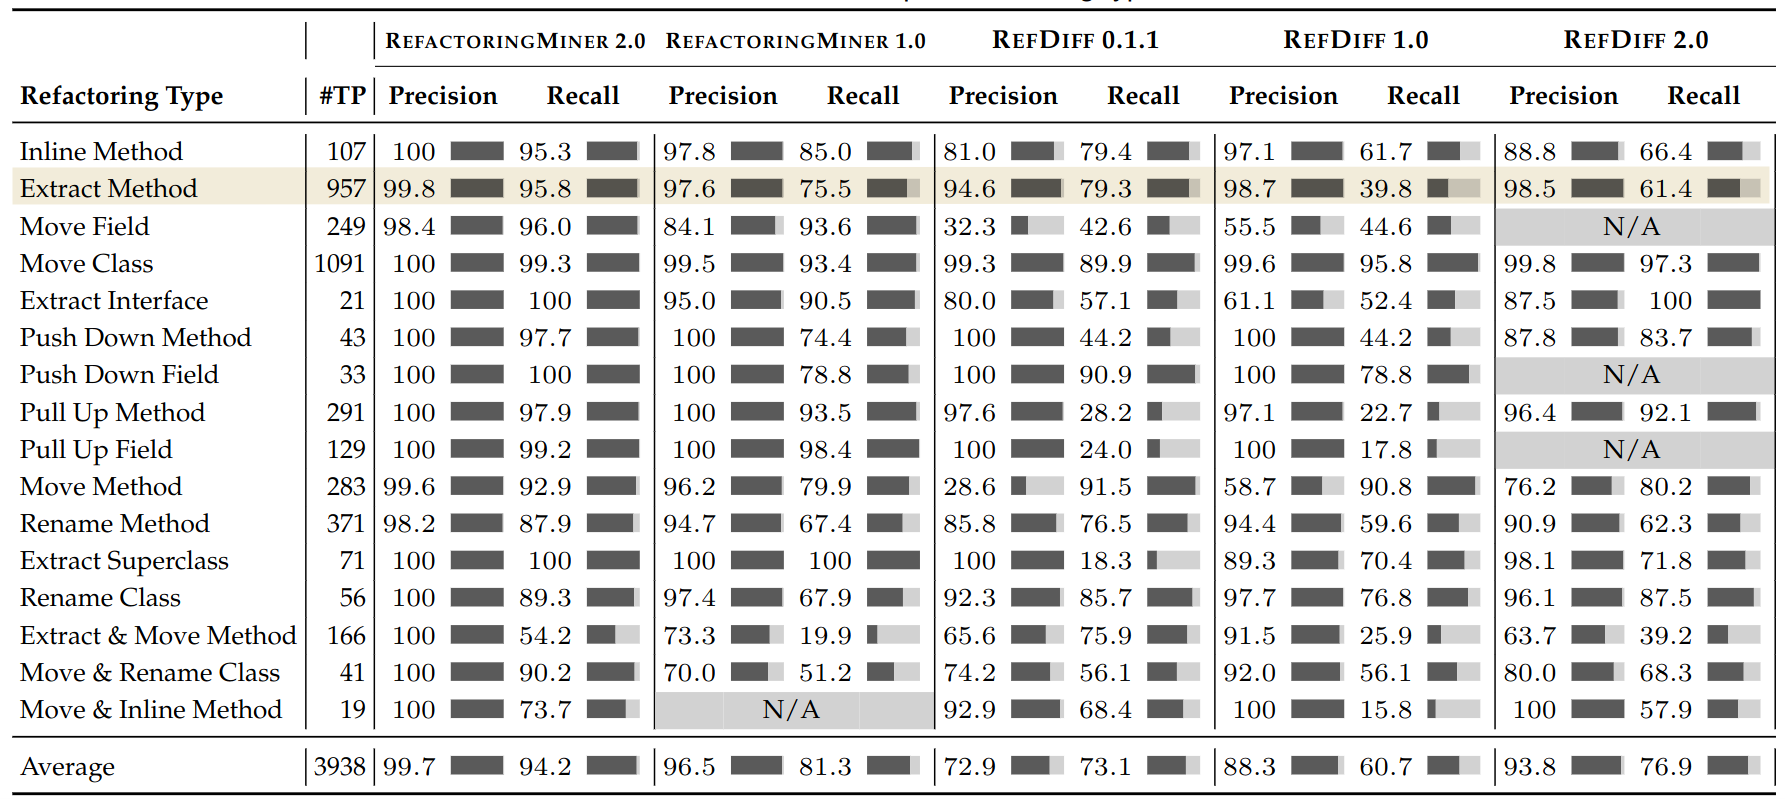
\includegraphics[width=\textwidth]{figuras/tabela_refminer_refdiff.png}   }
\caption{Precision and recall per refactoring type. Values calculated based on a refactoring
oracle of validated instances containing 7,226 true
positives in total, for 40 different refactoring types detected
by one (minimum) up to six (maximum) different tools. Table  and caption from \citet{refactoringminer_2.0}, our highlight.}
\label{img:tabela_refminer_refdiff}
\end{table}

\begin{table}[!ht]
\centerline{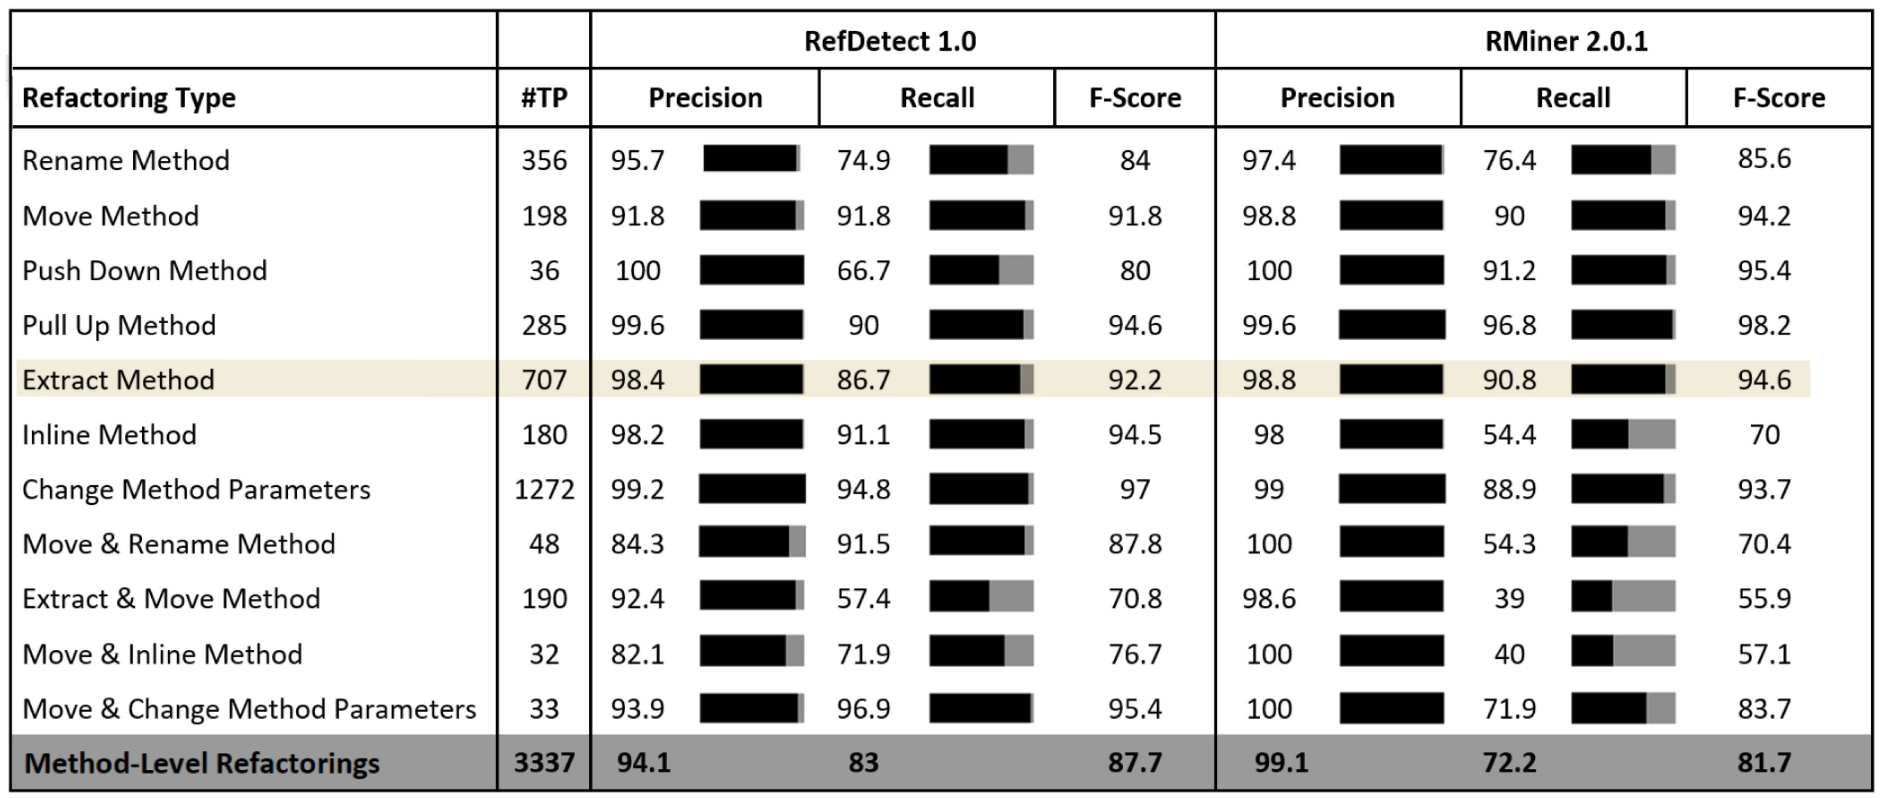
\includegraphics[width=\textwidth]{figuras/tabela_refdetect_refacminer.png}   }
\caption{Precision, recall and f-score results per method-level refactoring type. Values calculated based on a refactoring
oracle of validated instances from \citet{refactoringminer_2.0}, containing 7,226 true
positives in total for 40 different refactoring types detected
by one (minimum) up to six (maximum) different tools. Table from \citet{moghadam2021refdetect}, our highlight.}
\label{img:tabela_refdetect_refacminer}
\end{table}


With this, we also decided to utilize RefactoringMiner to build our dataset, but if in future work we expand on the refactorings we deal with or the targeted programming languages, RefDetect, a multilingual refactoring detection tool, may be a better pick:  

\begin{myquote}
\textit{RefDetect clearly outperformed R\textbf{(efactoring)}Miner in method and class based refactorings, achieving f-scores respectively of 87.7\% vs. 81.7\% for method-level refactorings and 92.1\% vs. 86.9\% for class-level refactorings.}
\\\citet{moghadam2021refdetect}
\end{myquote}


\section{Pipeline}

The overall structure of our pipeline is quite simple, as can be seen in Fig.~\ref{pipeline}. We start by cloning over 40.000 repositories of Java projects, these projects come from a list curated by the SERG group of the TUDelft university and available at \citet{lista_repos}.
With the repositories cloned we can start mining refactorings with RefactoringMiner. 
RefactoringMiner outputs one json file per mined repository, so our next step is to process all these json files and filter only the relevant features into our SQLite database. For this project we are only interested in function extraction refactorings, so we drop every other refactoring found. Then we check if the function extraction found covers a continuous span of lines, and if they are not continuous if maybe only blank lines or comments separate the continuous chunks; Fig.~\ref{img:dfa} illustrates this process with a Discrete Finite Automata. Lastly, we exclude any refactorings that happen at the same function in a same git commit. We do so to simplify our model and training process, we believe keeping these refactorings would negatively impact our performance and raise an issue of non determinism since multiple predictions could be found to be correct.

\begin{figure}[!ht]
\centerline{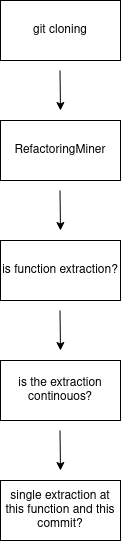
\includegraphics[scale=0.50]{pipeline.png}   }
\caption{A short visualization of the steps present in our data pipeline.}
\label{pipeline}
\end{figure}


The entirety of the code utilized in the construction of this dataset is available in Appendix~\ref{an:code_data}.




\begin{figure}[!ht]
\centerline{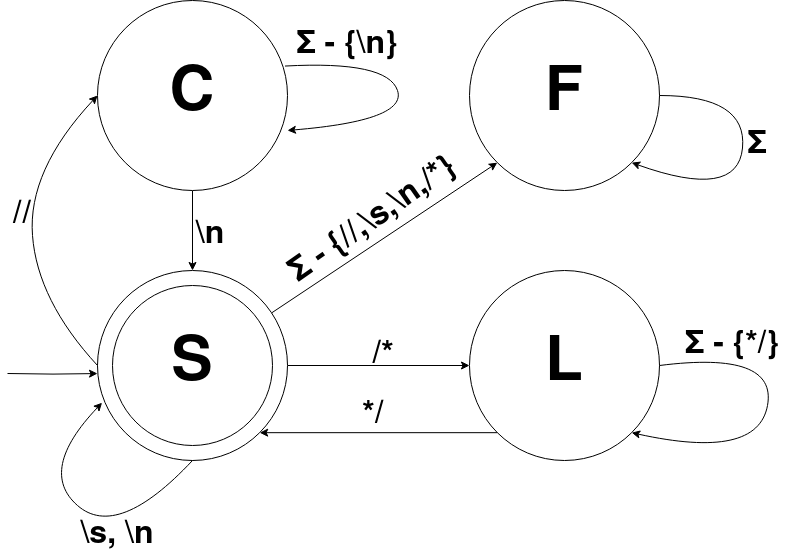
\includegraphics[width=0.6\textwidth]{figuras/DFA.png}   }
\caption{A Discrete Finite Automata that detects if any of the lines analyzed is not a comment or blank line. For the sake of simplicity and illustration, let us consider that symbols such as ``//'', ``/*'', ``*/'', ``\textbackslash n'' and ``\textbackslash s'' are single characters. Building a real DFA that breaks each of these ``signals'' into their constituent characters would increase the complexity of the system and loose its meaning as an illustration to clarify our data processing.
Following convention, $\Sigma$ represents the alphabet of this DFA, i.e. the set of all valid characters in the java language. State \textbf{S} represents blank lines, the \textbf{C} state represents comments and \textbf{L} long comments, lastly the \textbf{F} state represents a failure, once something that does not constitute a comment, long comment or blank line is detected the process gets stuck in the \textbf{F} state unable to ever reach the accepting state 
\textbf{S}.}
\label{img:dfa}
\end{figure}

\section{Exploration of the dataset}

Even though we started with a list of 49,982 Java repositories, we only managed to obtain function extractions from 19,936 of them. Many factors played a part in this, such as problematic encodings when processing the files, repositories not found due to renaming or migration, RefactoringMiner limitations, only refactorings other than function extraction found or even repositories that weren't purely written in Java (some were mostly written in Kotlin with just a few files in Java, for example).

However, even with all these issues we obtained 523,667 different instances of function extraction, an increase of over 60\% in comparison with the dataset we originally intended to use from \citet{mauricio_paper}. Interestingly, over 80\% of the function extractions found  are continuous, given the diverse range of Java projects used in this analysis we believe this should be a good approximation to the real proportion of continuous function extractions in relation to non-continuous. This further solidified our decision to focus on only continuous extractions for our model, since they are not only simpler to train but also arguably a more useful and actionable suggestion for developers.


